%!TEX root = ../dissertation.tex
\chapter{Industrial Use Case}
\label{industrial-use-case}

In this chapter will be presented a use case for the developed sentiment analysis model. For an initial test have been crawled new data focused on the target subject, and after been processed for the sentiment classification, have been presented with the Oracle Data Visualization Desktop tool. In the following paragraphs it will be discussed all the followed steps, and finally some information that have been extracted from the data.

\section{New Data Gathering}

For a preliminary use case of the sentiment analysis classification model discussed so far, it has been decided to introduce new information reputed useful for marketing analyses, with respect to the ones discussed for the yet gathered dataset. The whole information downloaded in the new crawling were:
\begin{itemize}
	\item Forum's name;
	\item URL;
	\item Thread's title;
	\item Comment's timestamp;
	\item User's total number of comments;
	\item User's subscription date;
	\item Text;
	\item Quote.
\end{itemize}

The procedure was the same followed for the gathering of the training dataset. However, for this purpose, the only comments that matter are the ones with a reference to the brand Porsche, so only comments belonging to Porsche's discussions were crawled. For future works, comments are supposed to be crawled from every kind of discussion, detecting automatically the pertinence to the target brand.\\
Some basic statistics about crawled comments are shown in Figure \ref{table:new-comments-test}.

\begin{table}[H]
	\centering
	\begin{tabular}{ | c | c | c | } 
		\hline
		Forum & \# Threads & \# Comments\\
		\hline
		Quattroruote & 12 & 473 \\
		\hline
		Bmwpassion & 8 & 883 \\
		\hline
		Porschemania & 37 & 5,039 \\
		\hline
		\hline
		TOTAL & 57 & 6,395 \\
		\hline		
	\end{tabular}
	\caption{Distribution of new comments.}
	\label{table:new-comments-test}
\end{table}

The threads have been manually selected. Have been chosen the most discussed threads, including also the main discussions related to a car model. All the comments have been classified by the sentiment analysis classifiers, with respect to the "engine", "brand", "exteriors" and "support" topics. Naturally, since data have not been manually labeled, it is not possible to evaluate scores about the quality of the classification, but the only way to achieve it, is looking at the details of the comments, like in a real world application.\\
In the following paragraph it will show how data have been visualized, exploiting a powerful data visualization tool.


\section{Data Visualization}




\subsection{Preliminary Information about Sentiment expressed in the Forums}


\begin{figure}[H]
	\centering
	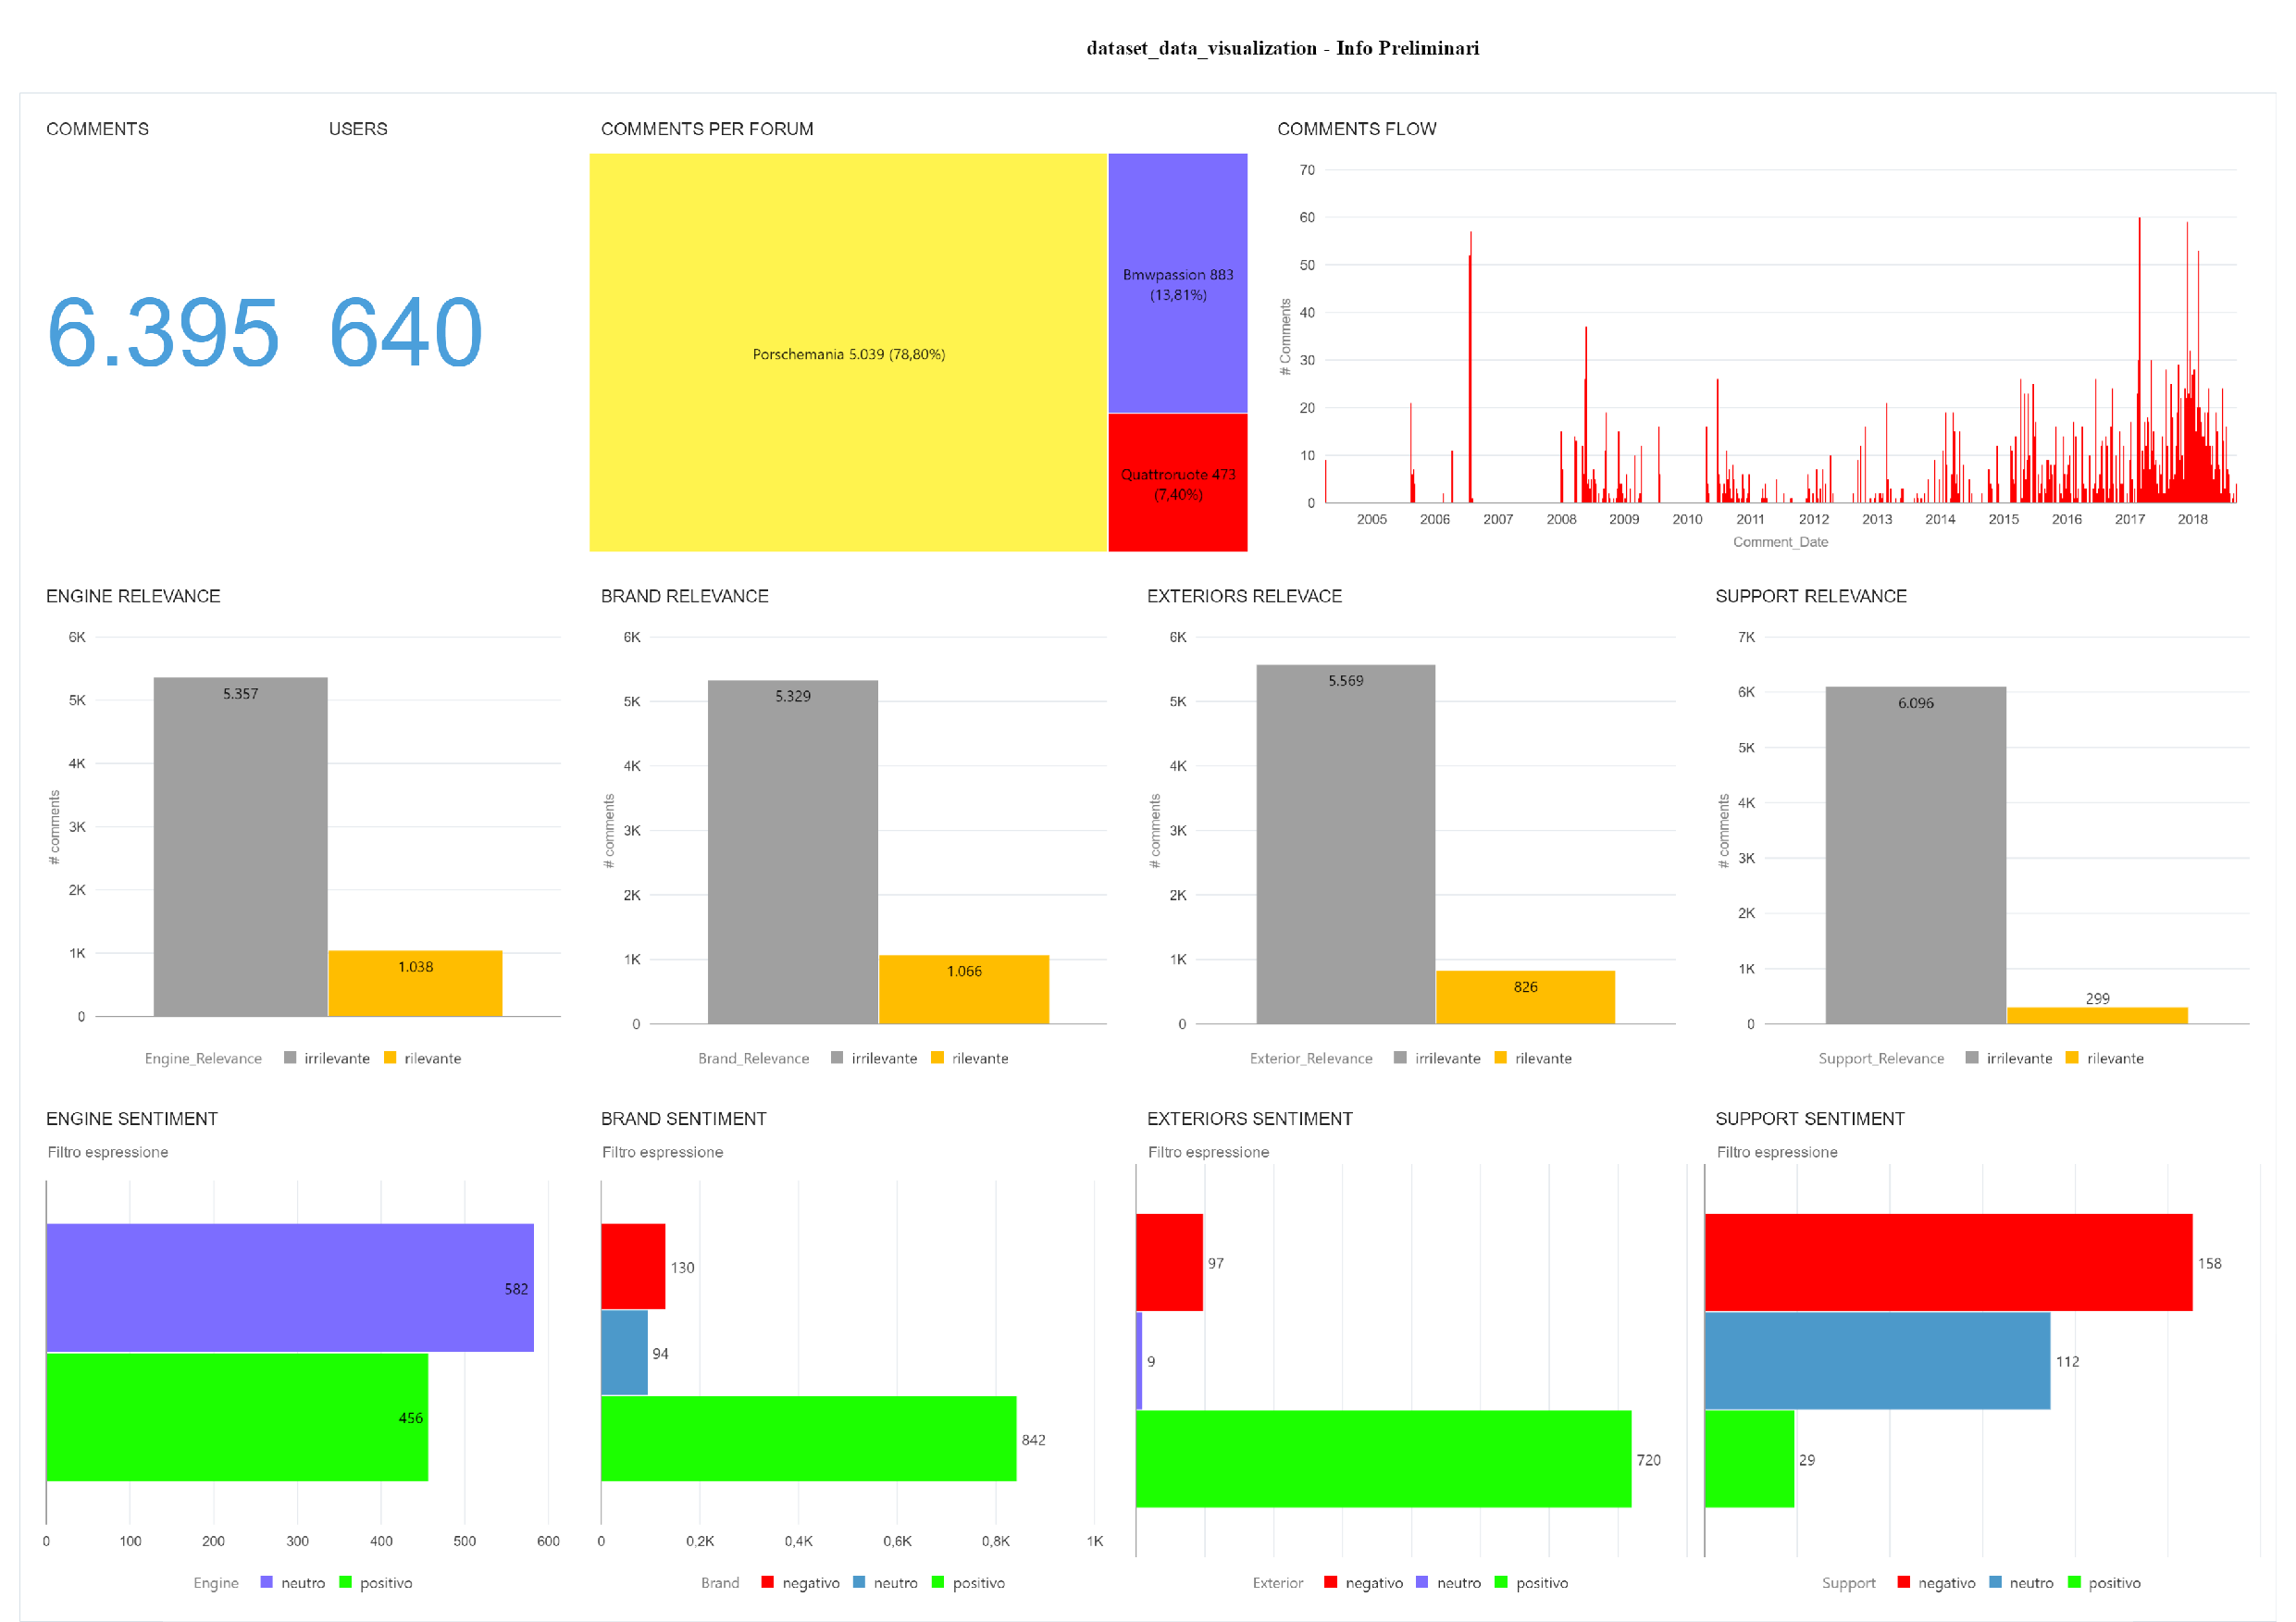
\includegraphics[width=\textwidth]{figures/odv_export/dataset_data_visualization_1.pdf}
	\caption{Overall statistics about the sentiment.}
	\label{fig:preliminar-info}
\end{figure}




\subsection{Sentiment Information about Porsche Panamera model}

\begin{figure}[ht]
	\centering
	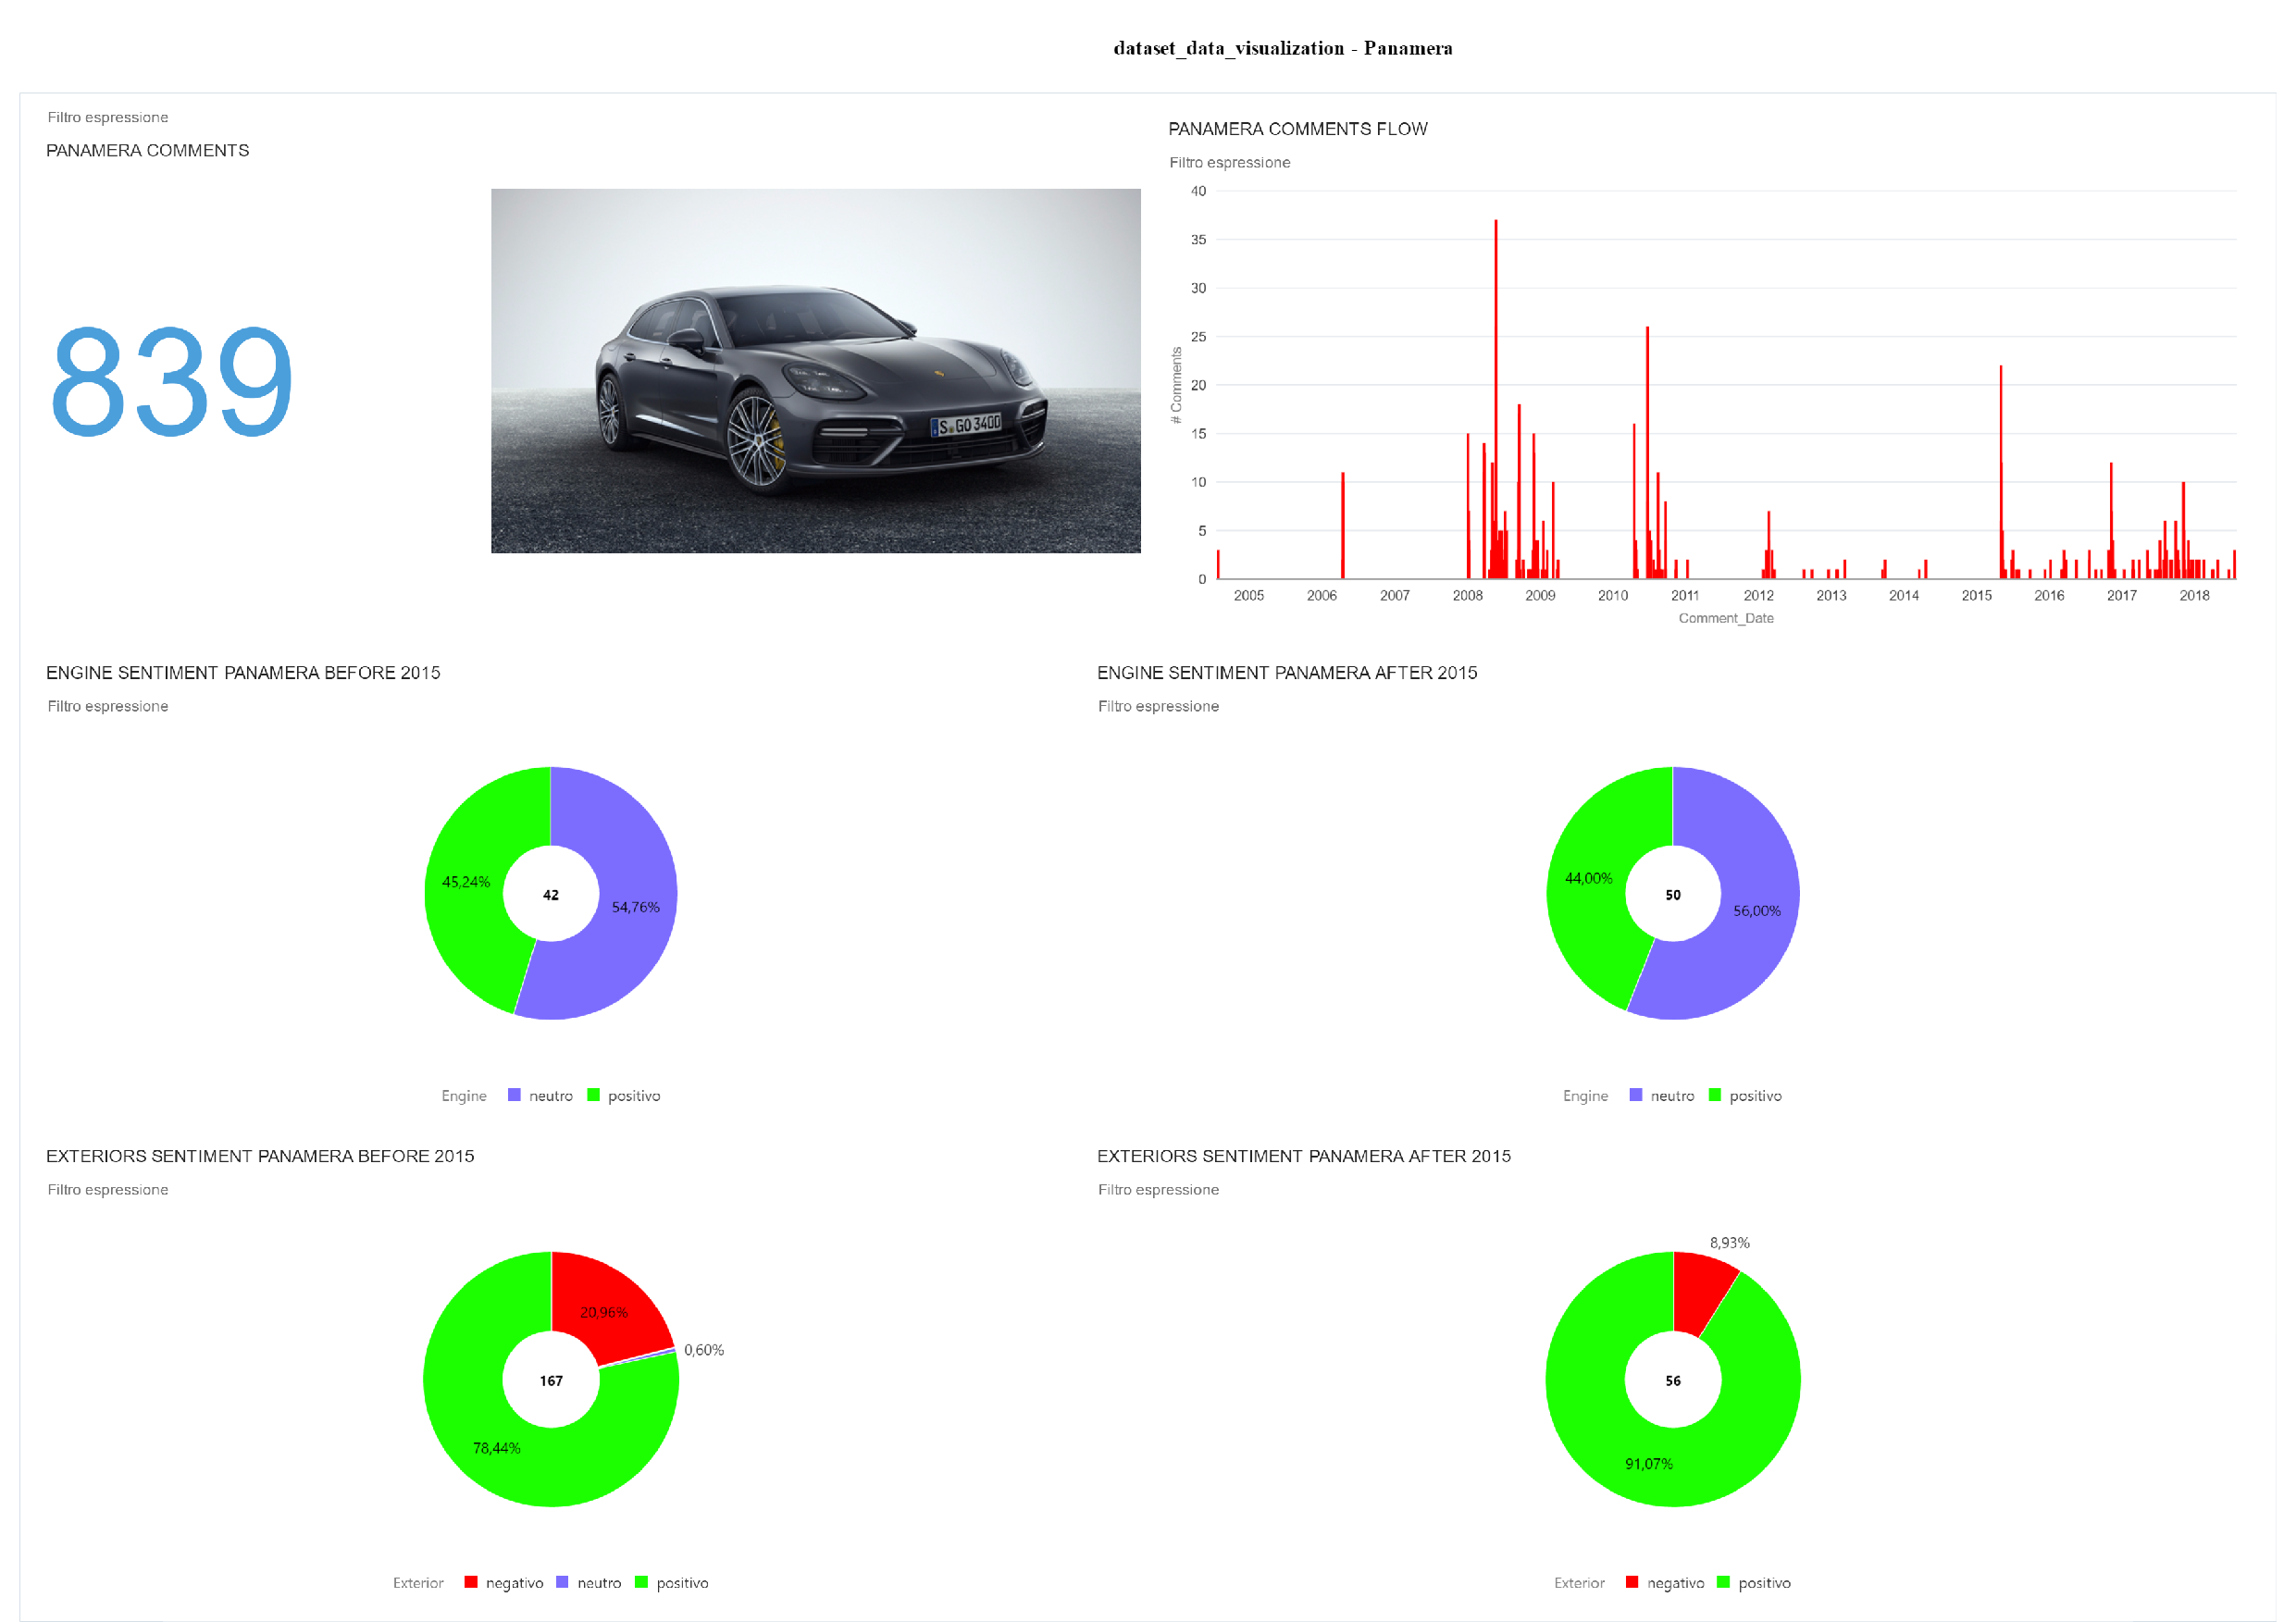
\includegraphics[width=\textwidth]{figures/odv_export/dataset_data_visualization_2.pdf}
	\caption{Sentiment polarities about Panamera model.}
	\label{fig:panamera-snt}
\end{figure}




\subsection{Sentiment Information about Porsche 911 (version 992) model}

\begin{figure}[H]
	\centering
	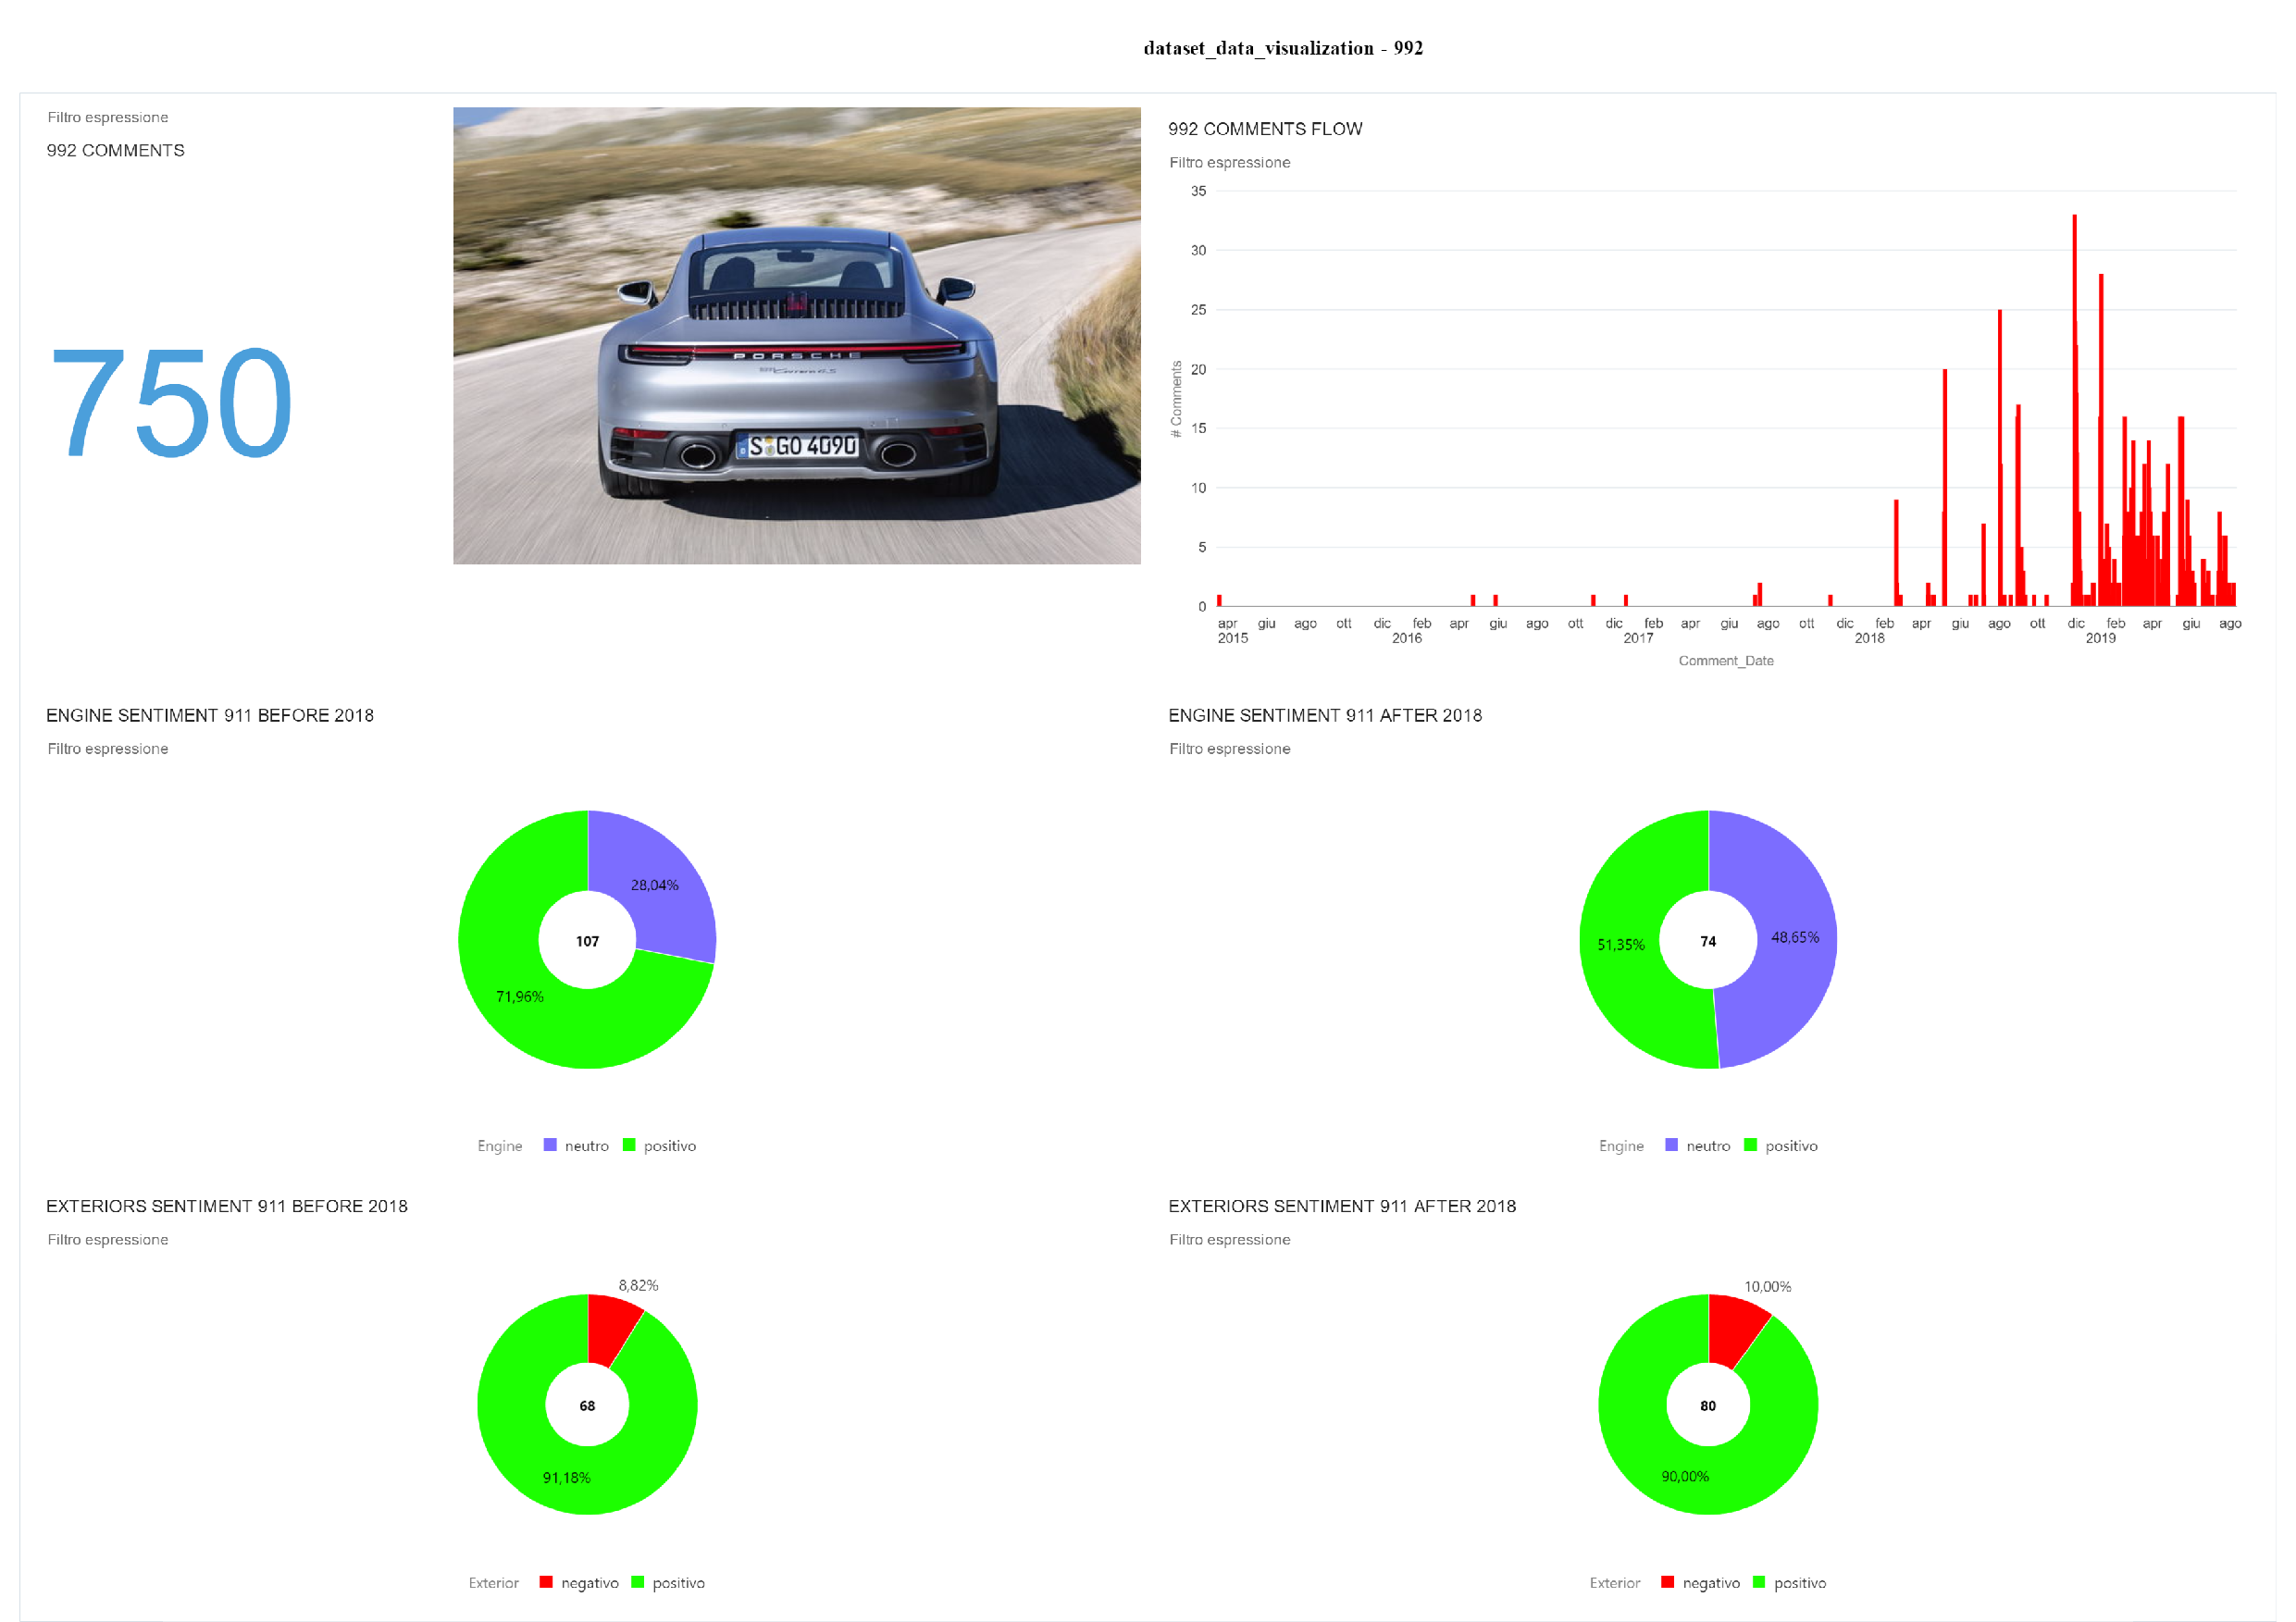
\includegraphics[width=\textwidth]{figures/odv_export/dataset_data_visualization_4.pdf}
	\caption{Sentiment polarities about 911 (992 version) model.}
	\label{fig:992-snt}
\end{figure}


\subsection{Sentiment Information about Cars' Exteriors}

\begin{figure}[H]
	\centering
	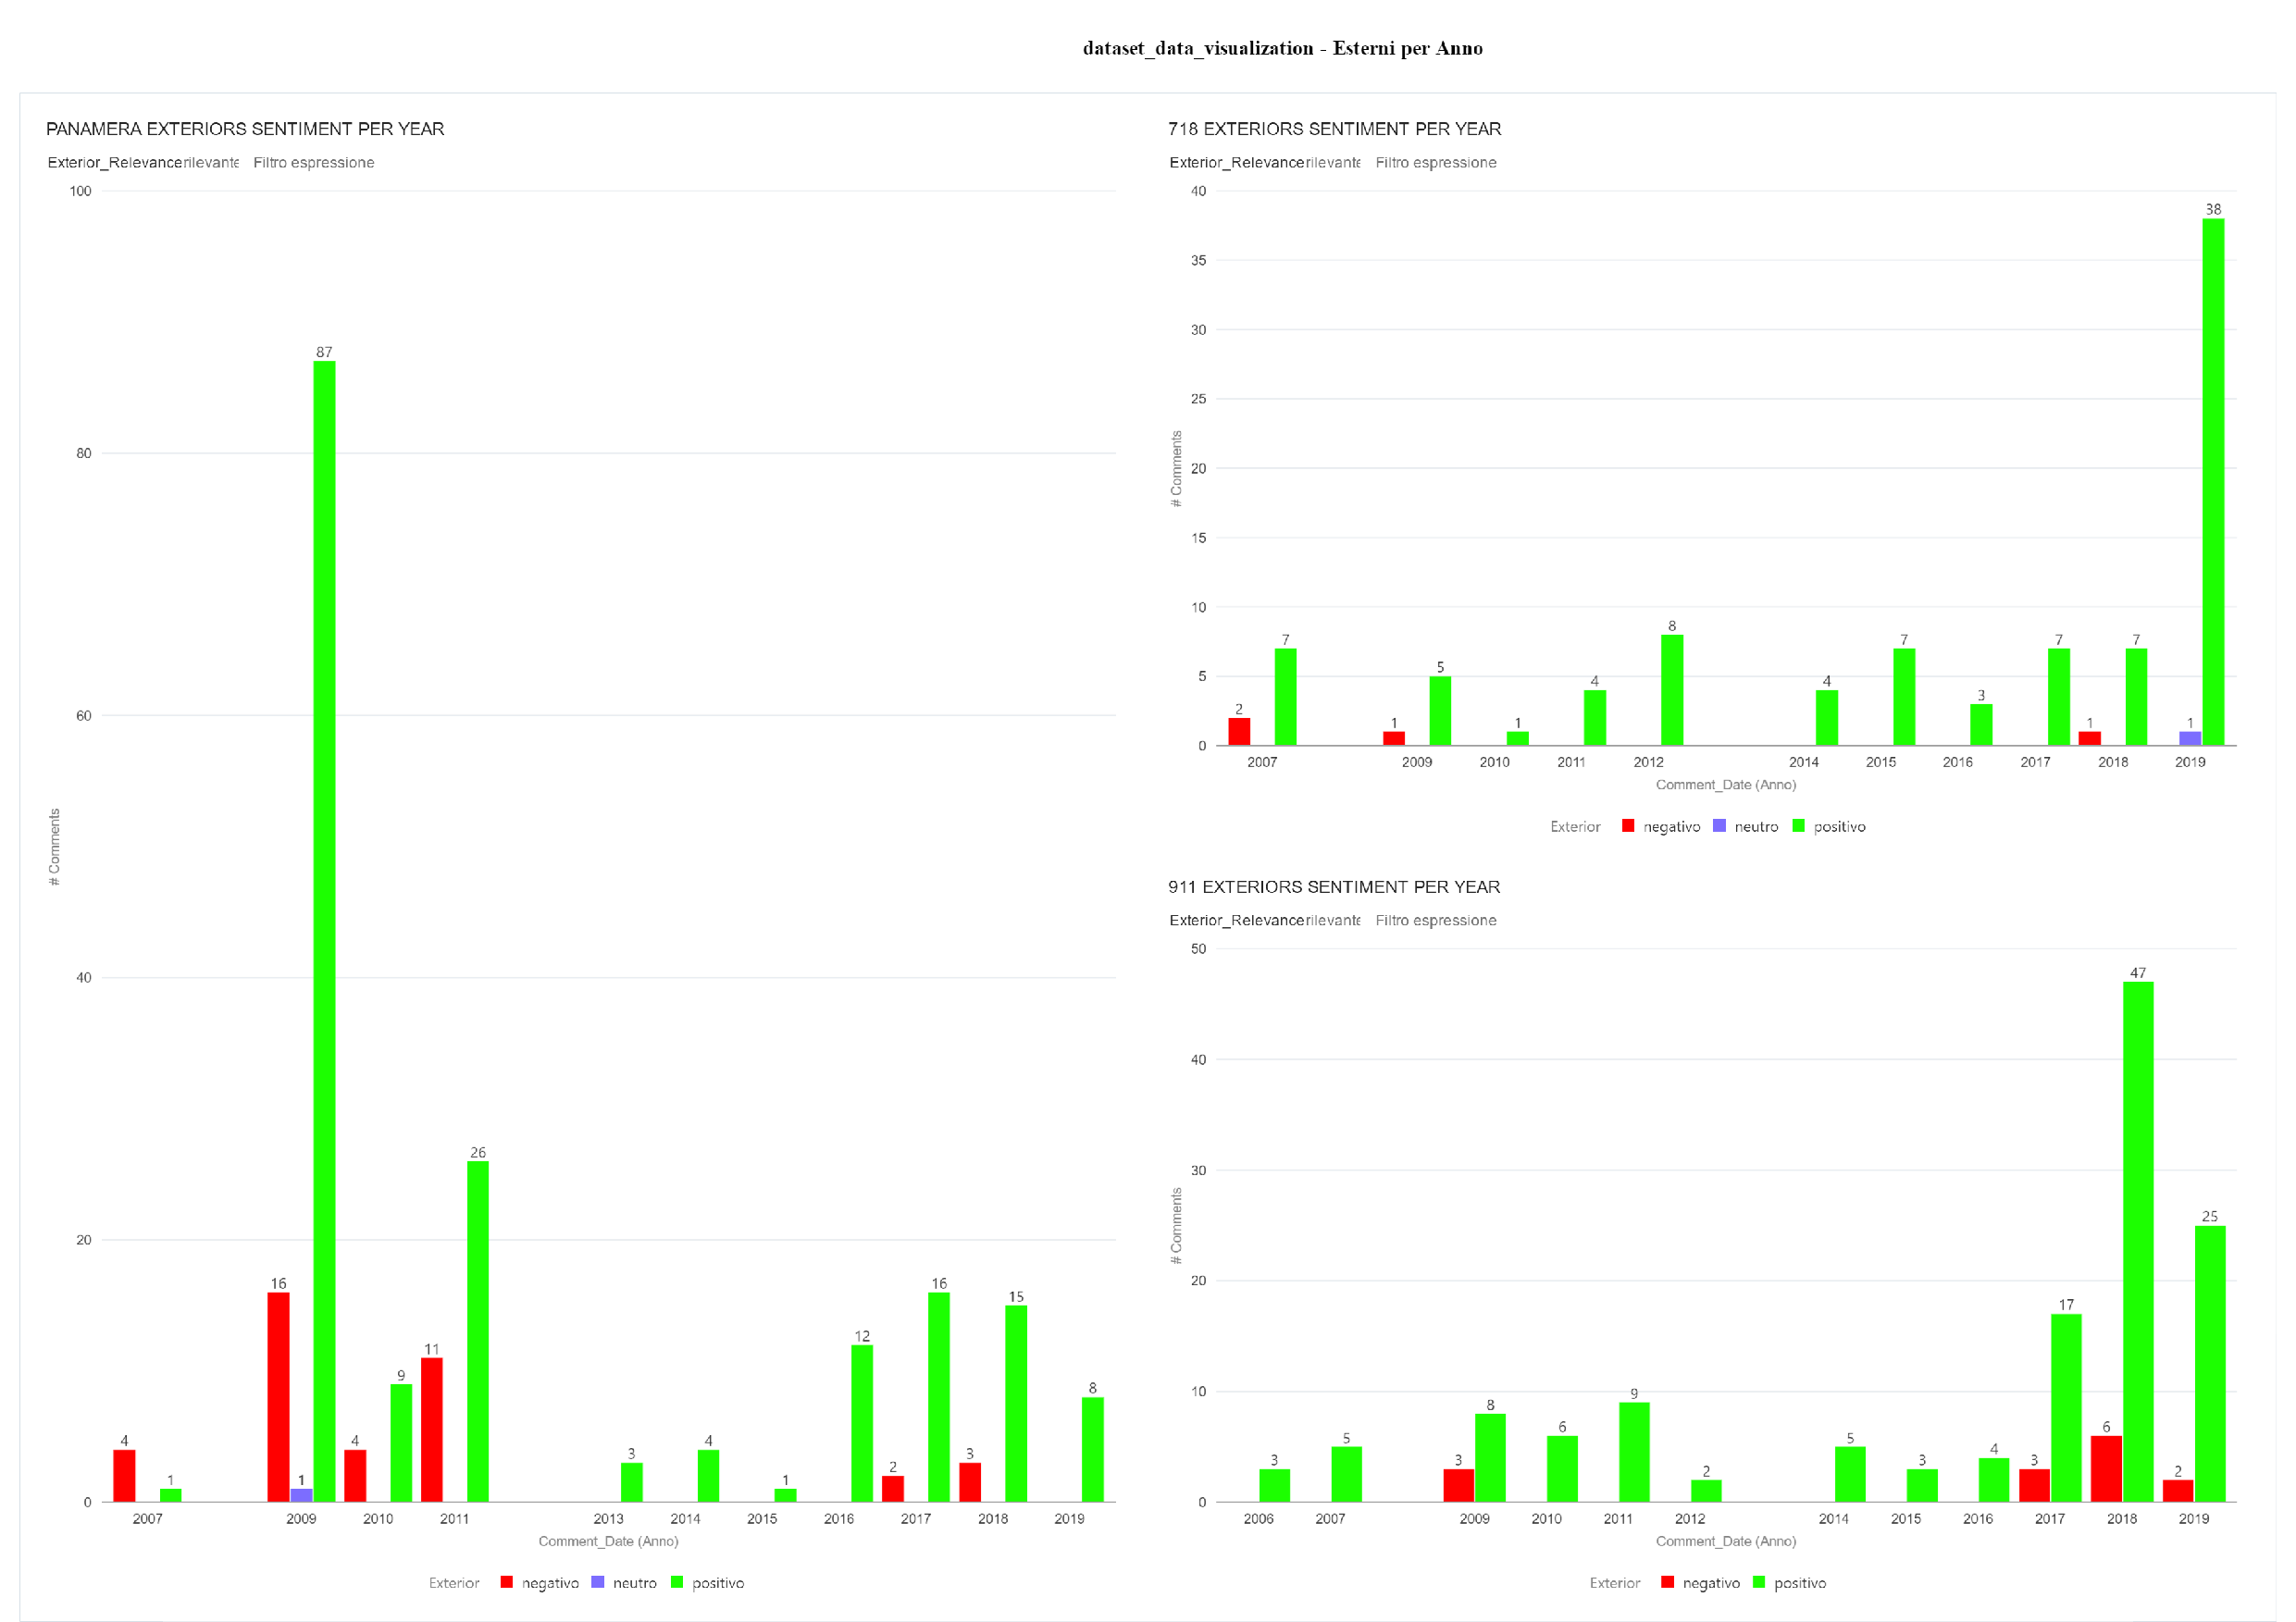
\includegraphics[width=\textwidth]{figures/odv_export/dataset_data_visualization_5.pdf}
	\caption{Sentiment polarities of some models on the years.}
	\label{fig:ext-year-snt}
\end{figure}



\subsection{Trend of Comments with respect to Users' Seniority}

\begin{figure}[H]
	\centering
	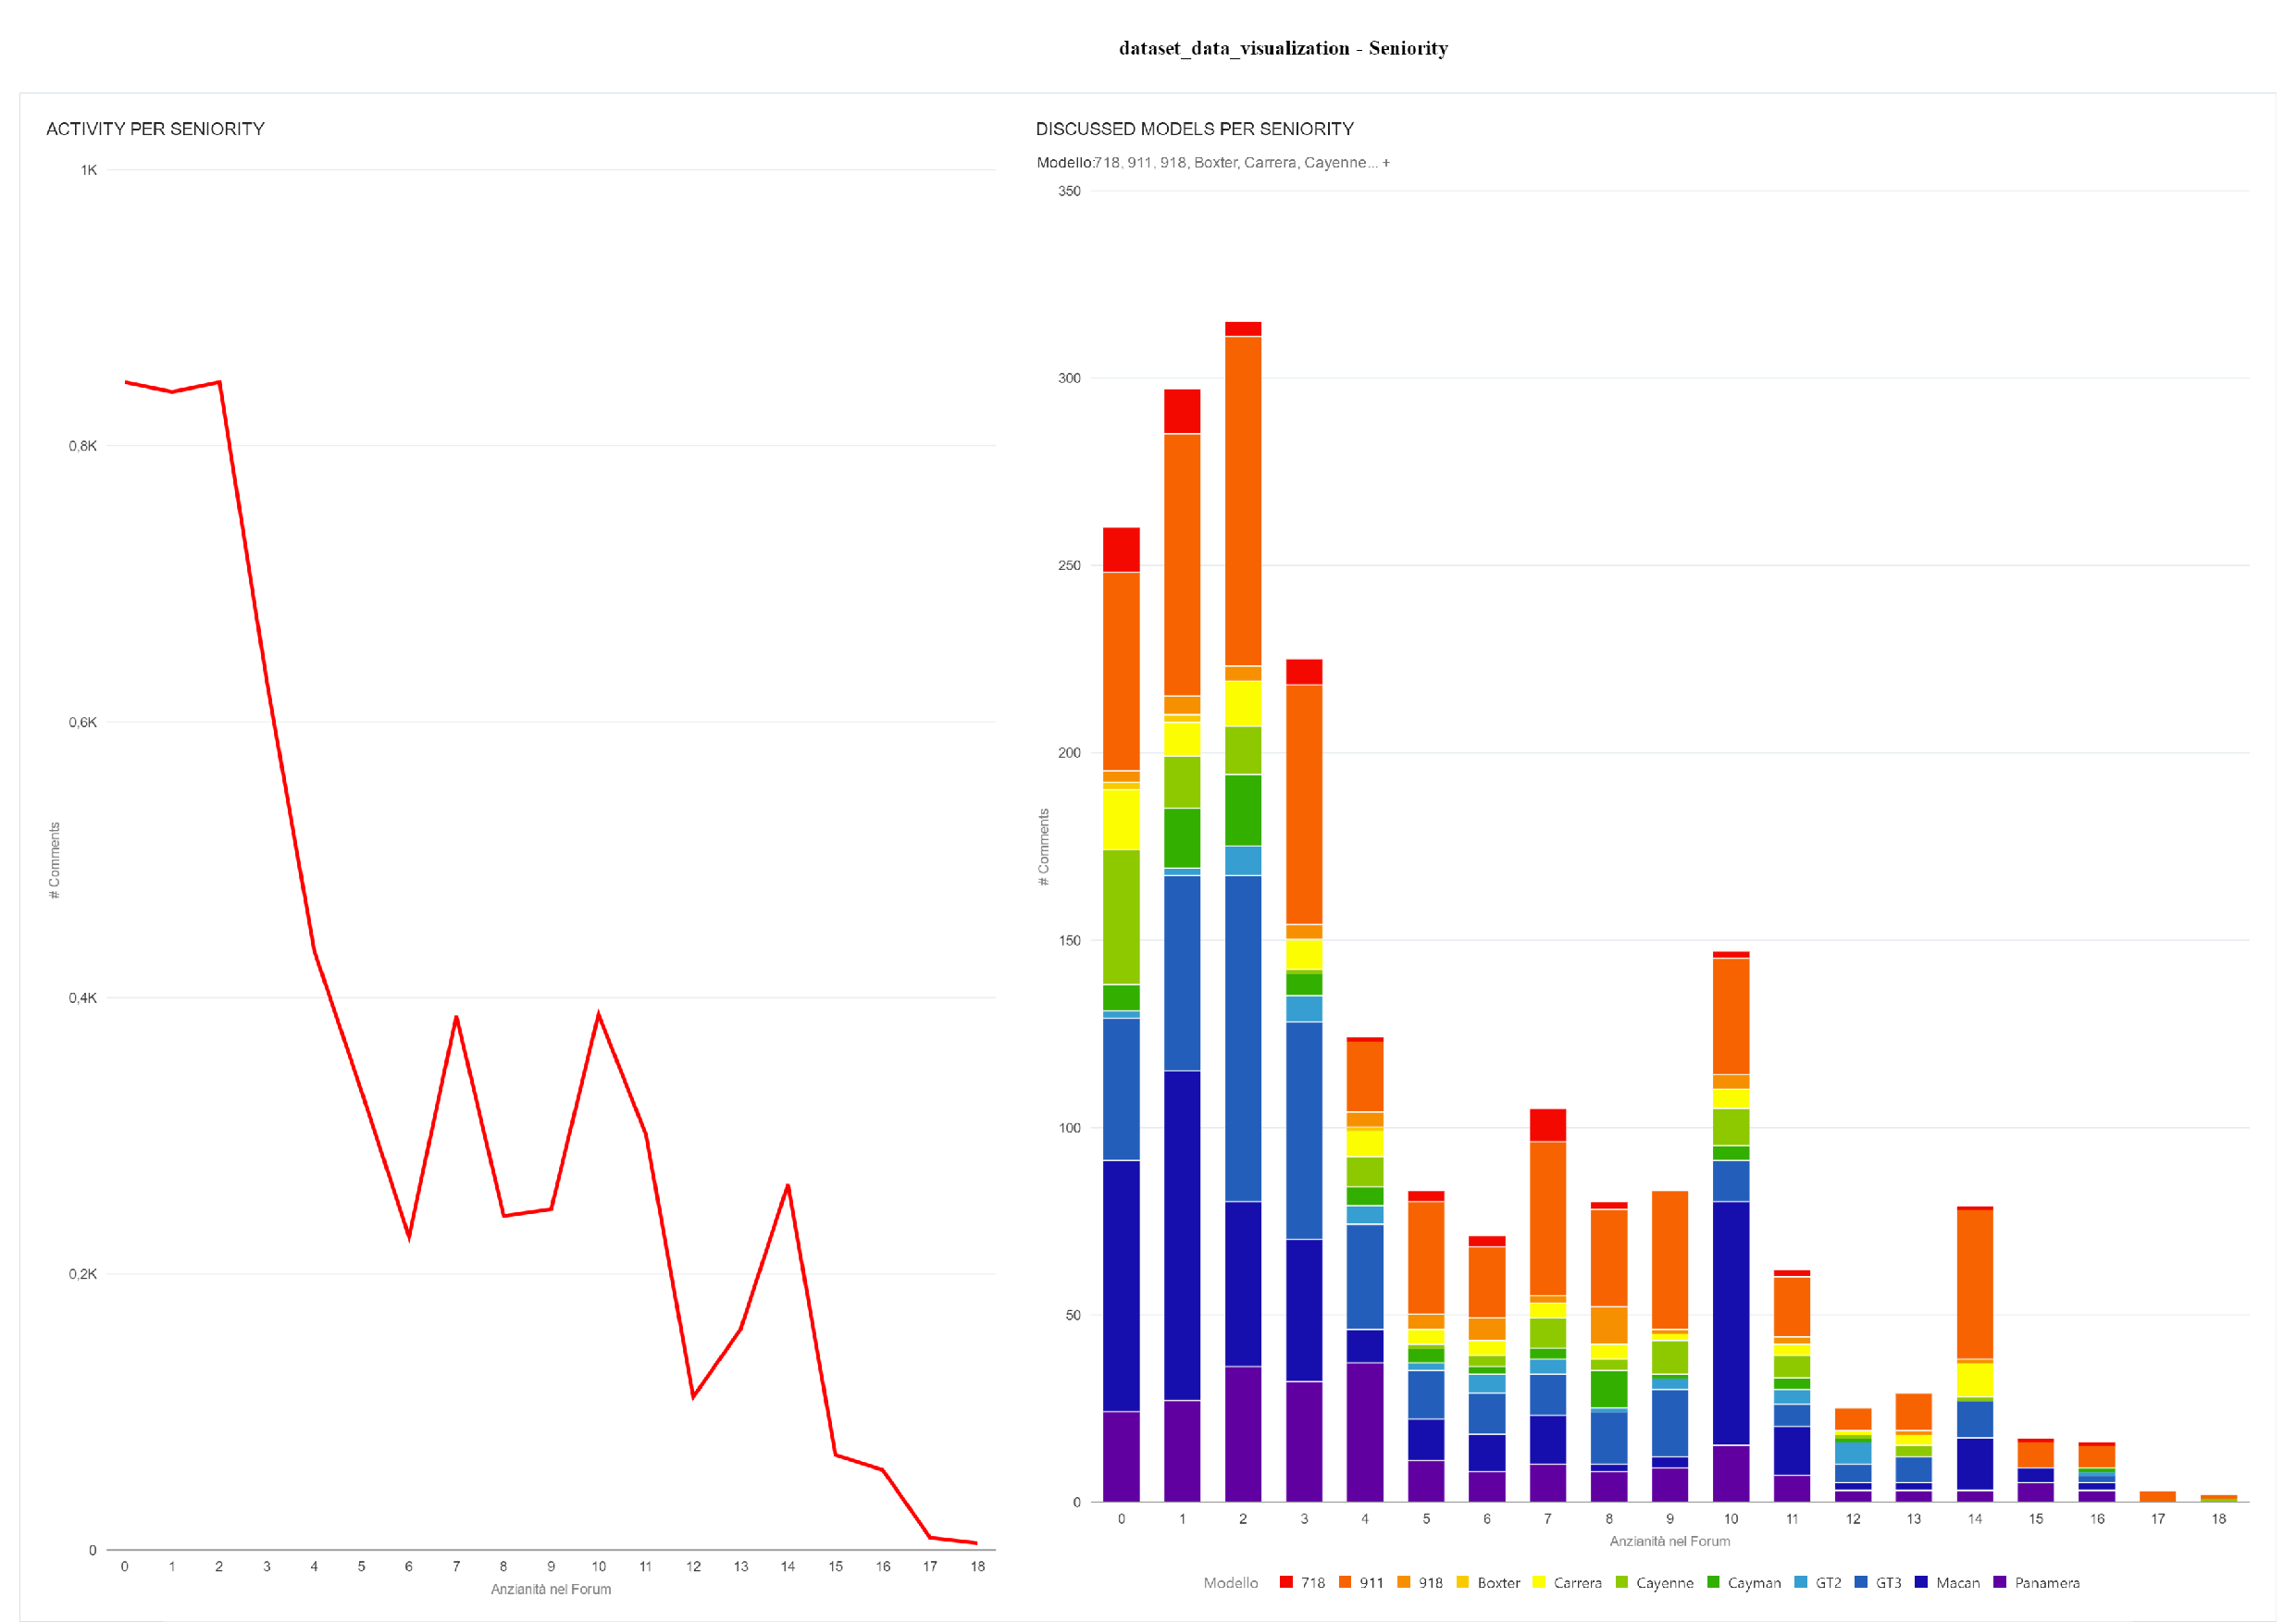
\includegraphics[width=\textwidth]{figures/odv_export/dataset_data_visualization_9.pdf}
	\caption{Models discussed per users' seniority.}
	\label{fig:model-senior}
\end{figure}




\subsection{Most discussed Models}

\begin{figure}[H]
	\centering
	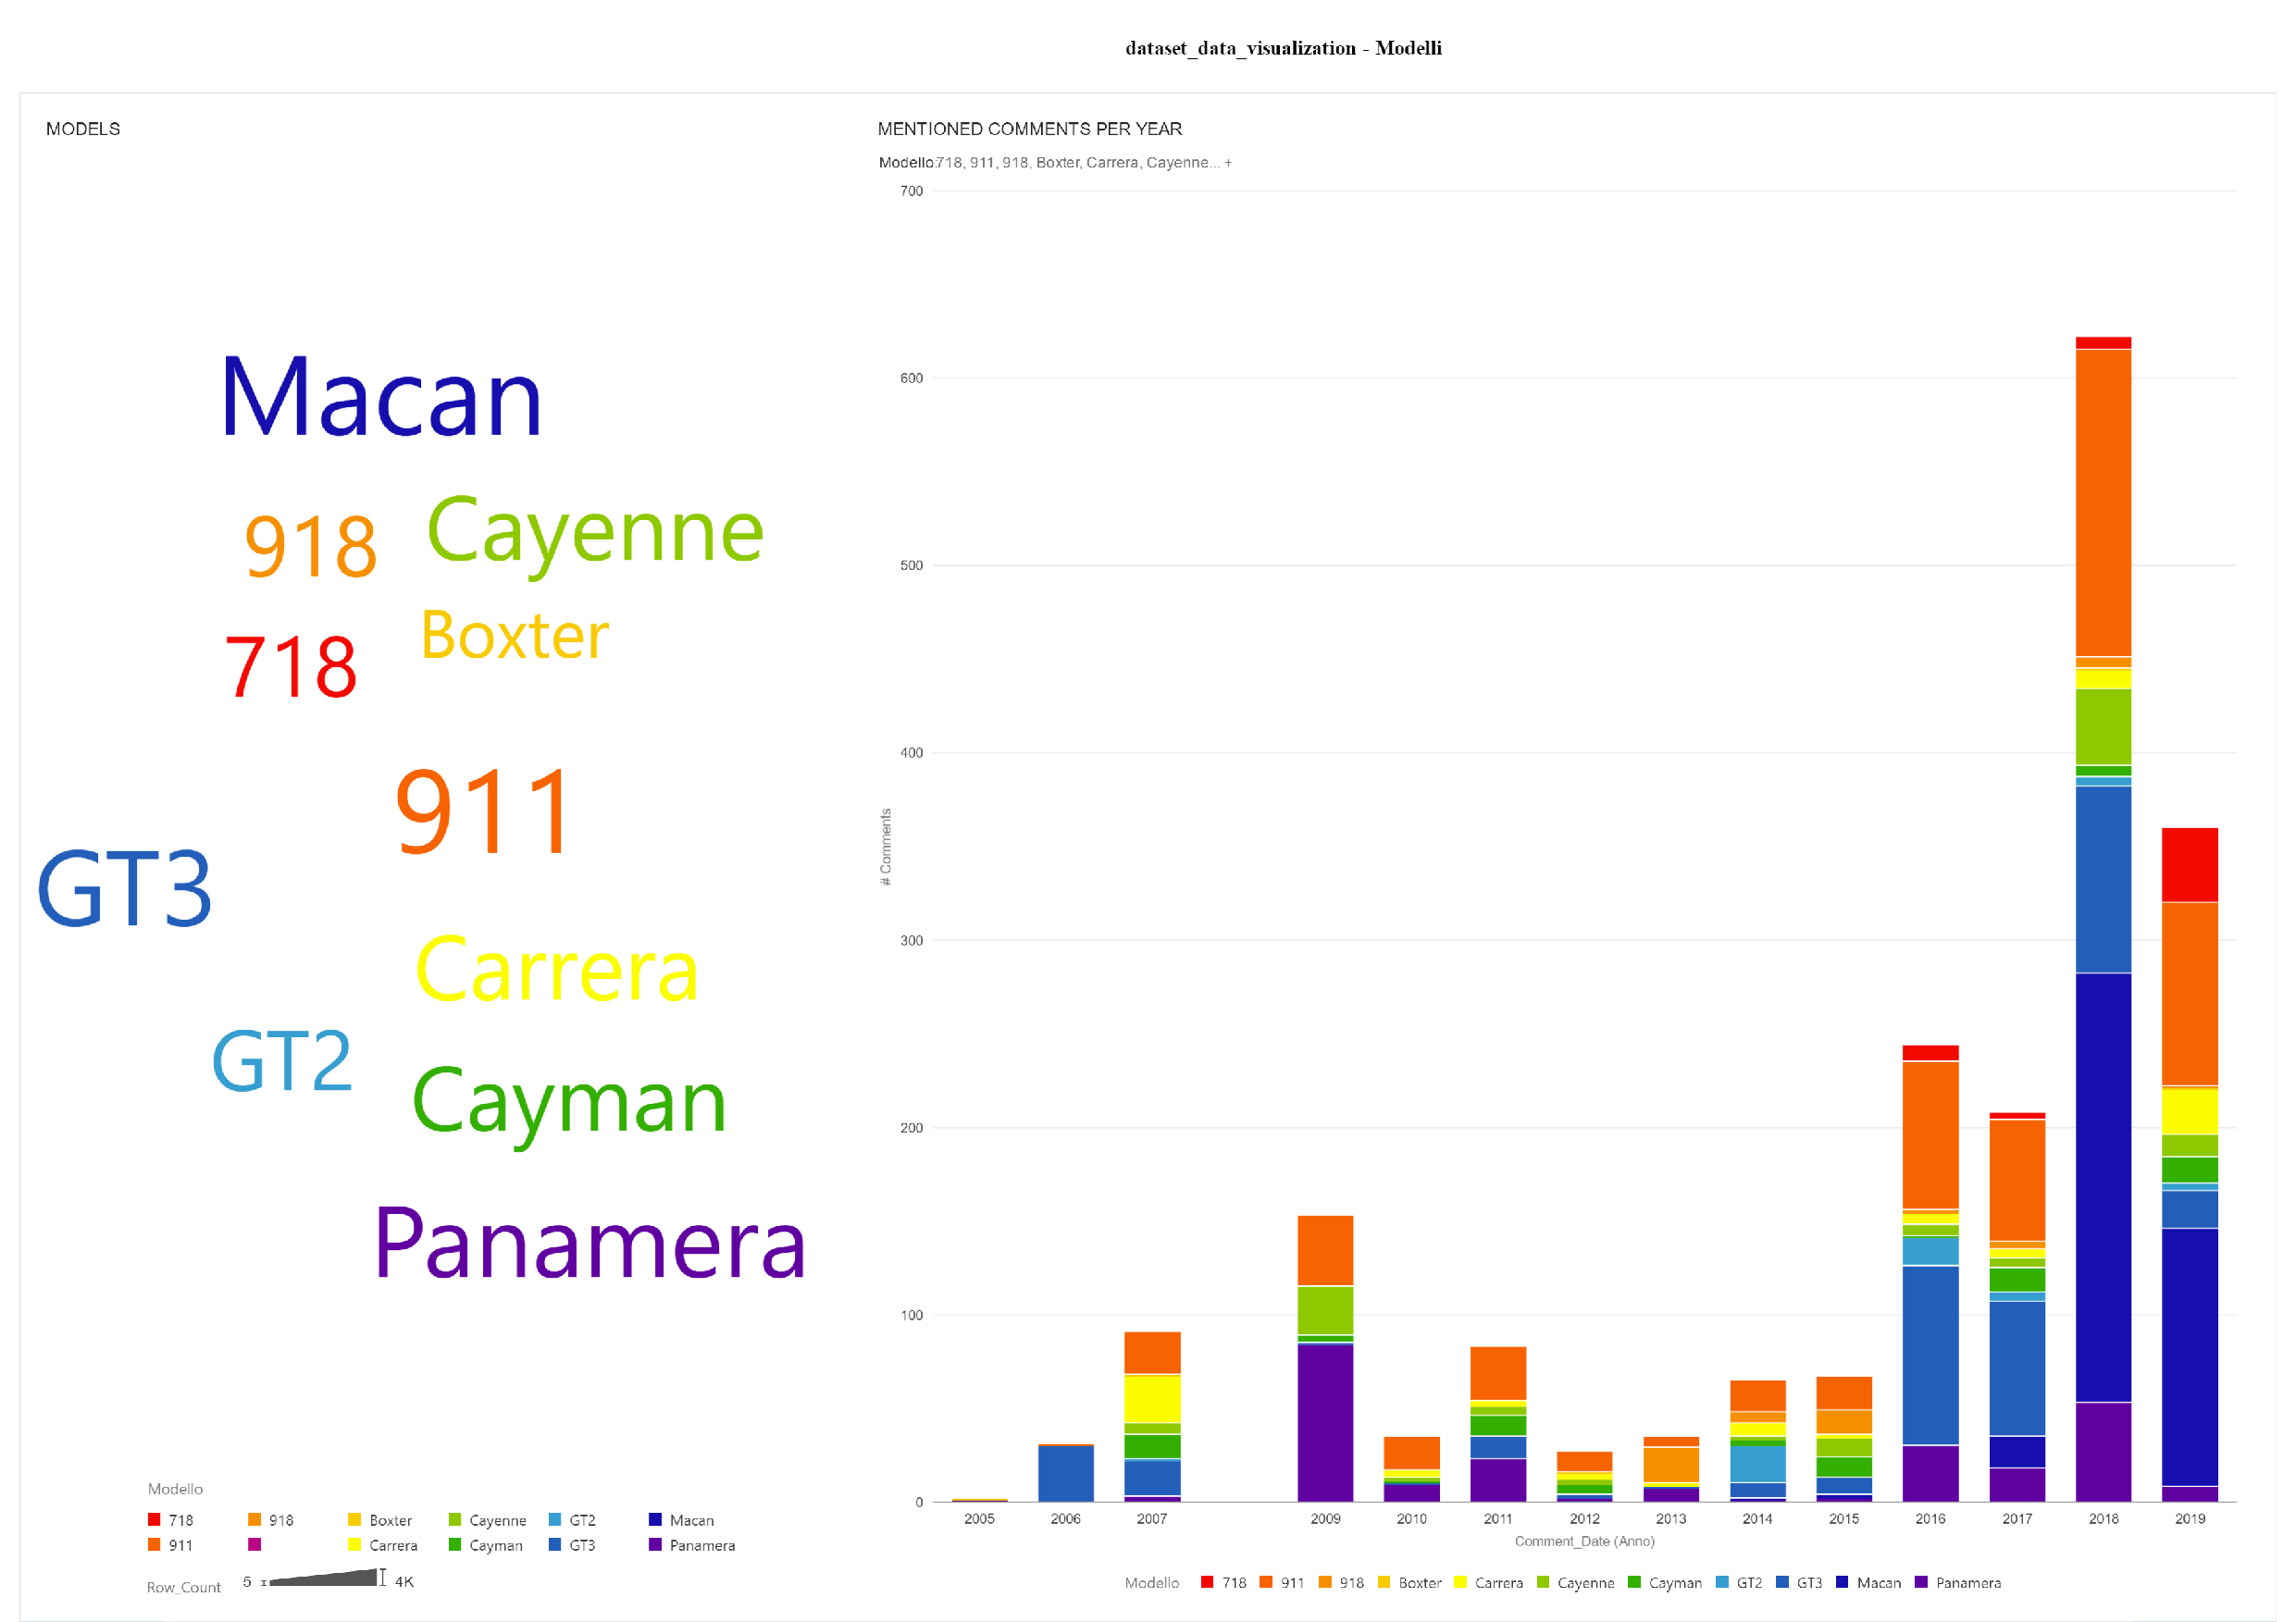
\includegraphics[width=\textwidth]{figures/odv_export/dataset_data_visualization_13.pdf}
	\caption{Most discussed models.}
	\label{fig:models}
\end{figure}